\section{\ours{}}
\label{sec:method}

\begin{figure*}[t]
    \centering
    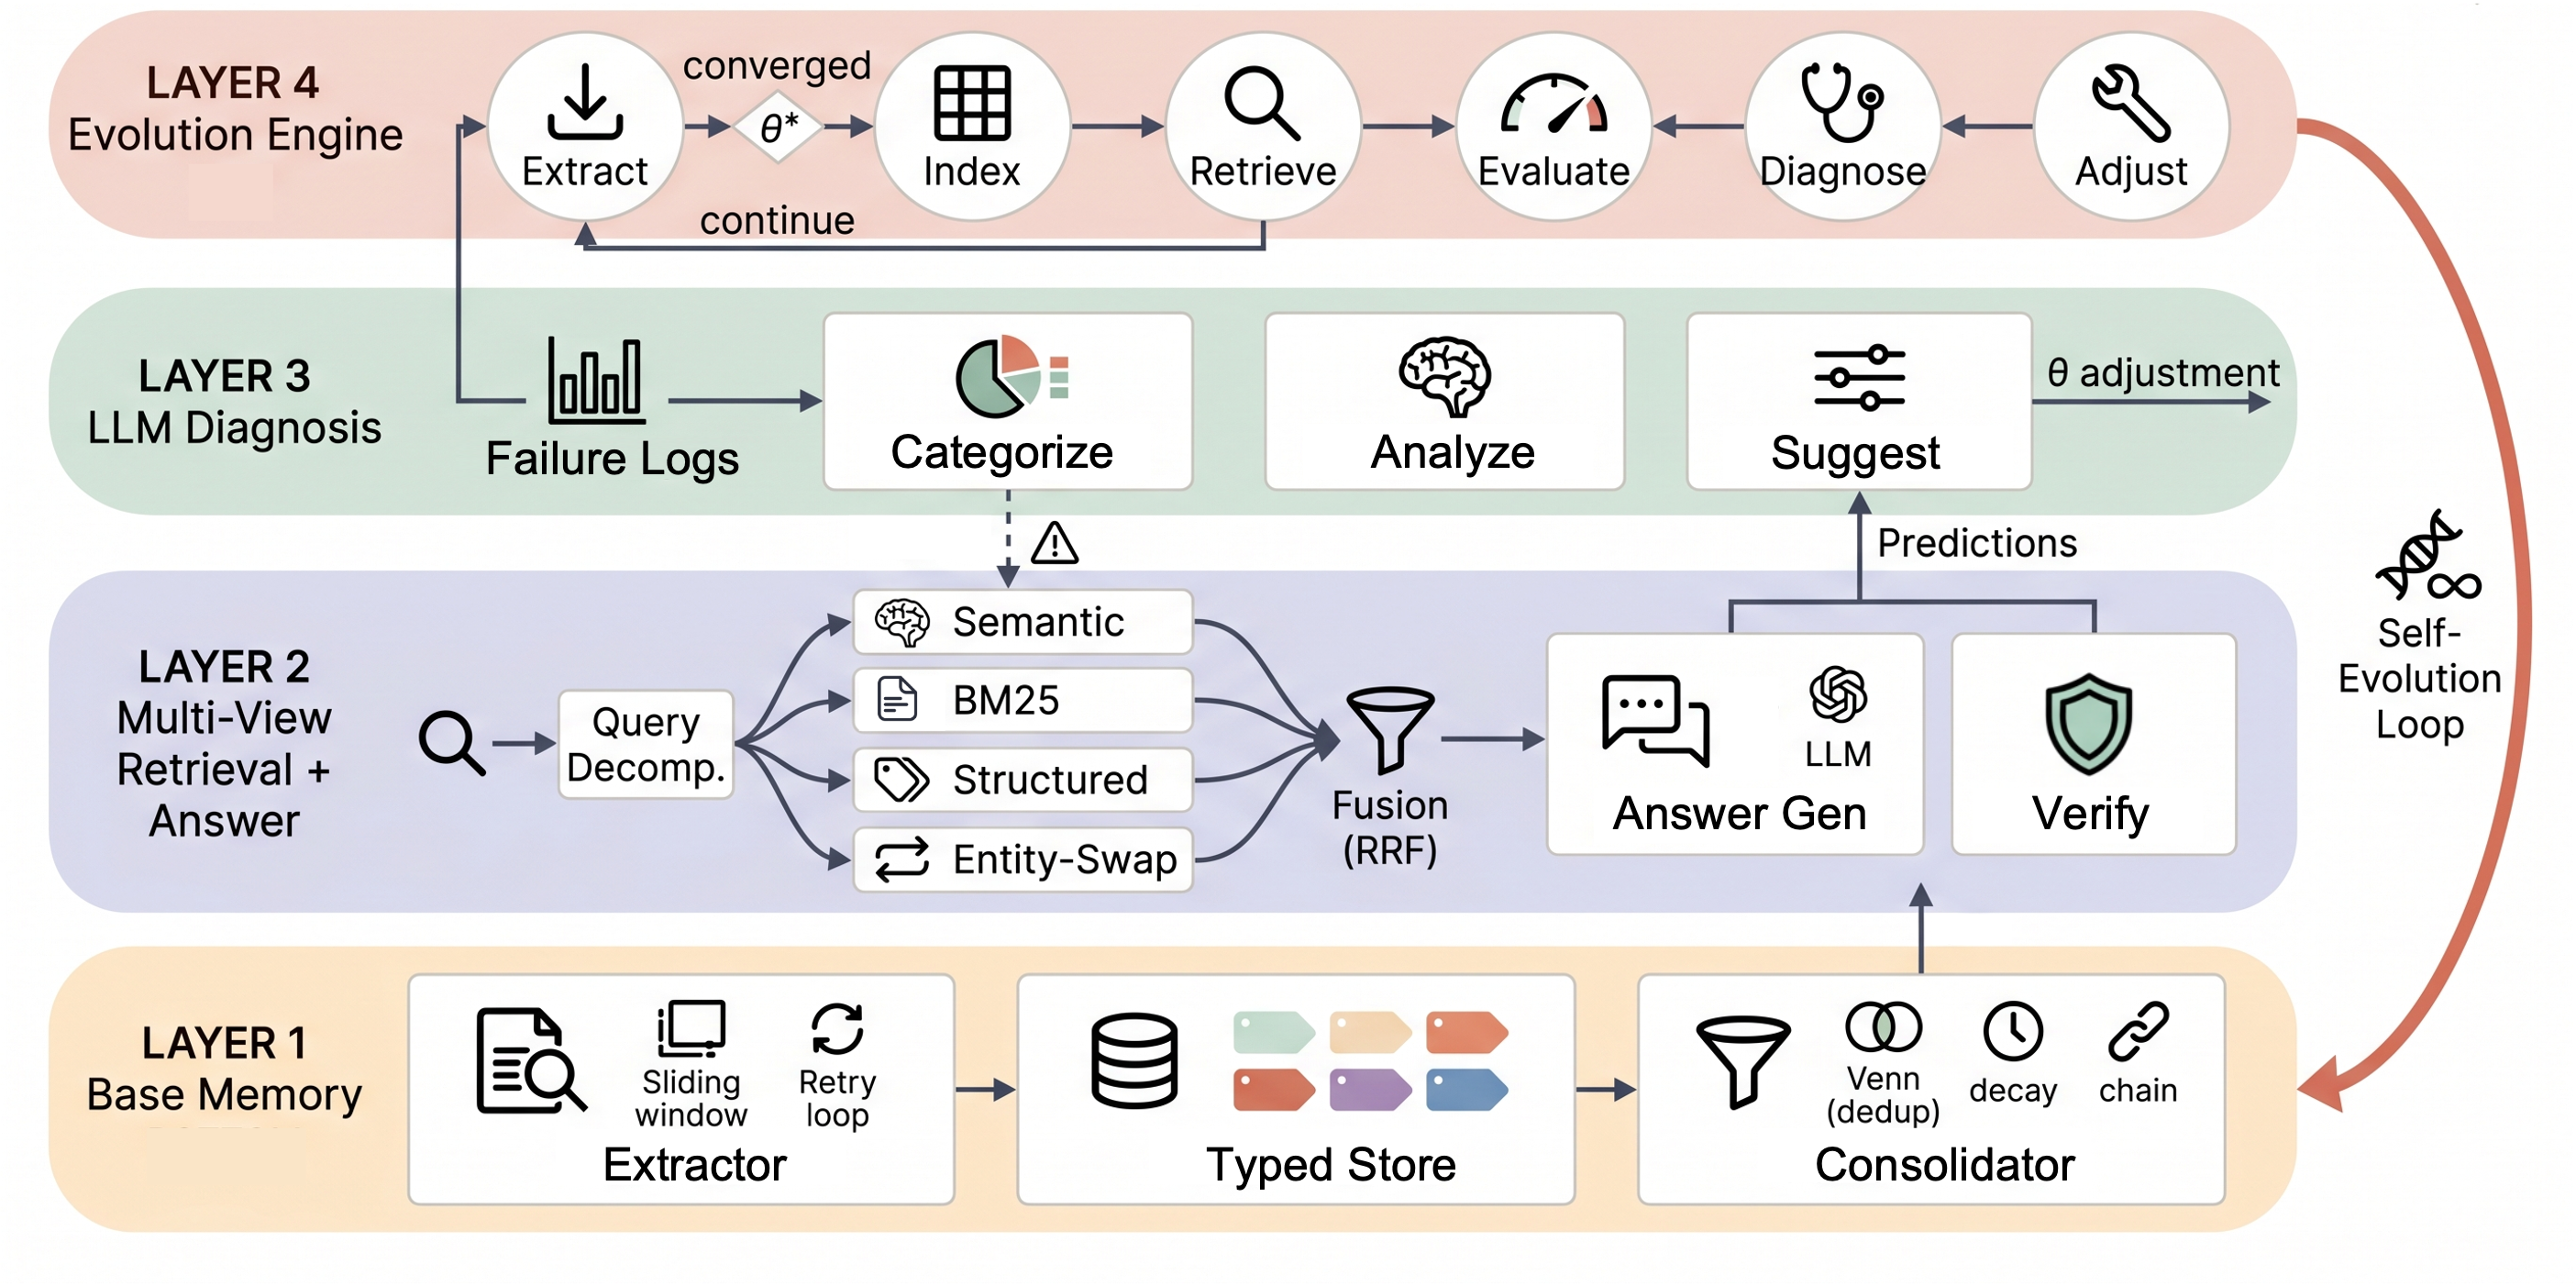
\includegraphics[width=\textwidth]{figs/framework.png}
    \caption{\textbf{\ours{} architecture.} Three layers connected by a self-evolution feedback loop. A typed memory store is populated by an LLM-based extractor with retry and chunk-splitting; a multi-view retriever fuses BM25, semantic, and structured-metadata search with optional entity-swap, query decomposition, and answer verification; an LLM-powered diagnosis module reads per-question raw-result logs and proposes structured adjustments to the retrieval configuration; the evolution engine validates adjustments and auto-converges when the primary metric plateaus.}
    \label{fig:architecture}
    \vspace{-1.5em}
\end{figure*}

The key design principle of \ours{} is that the retrieval infrastructure itself is a first-class optimization target, not a set of hand-tuned hyperparameters frozen at deployment time. Rather than relying on manual research to find good configurations, \ours{} automates the entire research process: it observes system behavior, diagnoses failure patterns, proposes architectural changes, and validates them empirically. As illustrated in Figure~\ref{fig:architecture}, three components realize this AutoResearch principle through a closed evolution loop. A \emph{Structured Memory Store} (\S\ref{sec:memory_layer}) builds and maintains a typed knowledge base through LLM-based extraction and consolidation. A \emph{Retrieval Layer} (\S\ref{sec:retrieval}) exposes its full configuration as an evolvable action space, enabling every parameter from fusion weights to answer generation style to be optimized jointly. A \emph{Self-Evolution Engine} (\S\ref{sec:evolution_engine}) closes the loop: it reads per-question failure logs, categorizes root causes, proposes targeted configuration adjustments, and applies them with safeguards against regression. This closed-loop self-evolution realizes an AutoResearch process, mirroring the observe-hypothesize-experiment-validate cycle of human research. Detailed formulations and threshold values are provided in Appendix~\ref{app:detailed_formulations}; the complete pipeline is given as Algorithm~\ref{alg:full_pipeline} in Appendix~\ref{app:full_algorithm}.

\subsection{Structured Memory Store}
\label{sec:memory_layer}

A self-evolving retrieval system is only as good as the memory it retrieves from. The memory layer provides a structured, high-quality knowledge base that supports multi-view retrieval across heterogeneous question types. This requires addressing three sub-problems: how to represent individual memories so that multiple retrieval views can operate over them, how to extract memories from raw conversations, and how to maintain store quality as memories accumulate over time.

\noindent \textbf{Memory representation.} Each memory unit is a tuple $m = (c,\; \mu,\; \mathbf{e},\; \boldsymbol{\eta}), \quad
\mu \in \mathcal{T},\; \mathbf{e} \in \mathbb{R}^d$, where $c$ is natural-language content, $\mathbf{e}$ is a dense embedding, $\mu$ is a memory type drawn from a six-category taxonomy $\mathcal{T}$ (covering episodic, semantic, preference, project state, working summary, and procedural knowledge), and $\boldsymbol{\eta}$ collects auxiliary metadata including importance, confidence, entity-reinforcement score, extracted entities (including persons and locations), topics, and creation timestamp.

\noindent \textbf{Memory extraction.} Given a source conversation $S = (u_1, \ldots, u_T)$, a sliding window of length $W$ partitions $S$ into overlapping segments. For each window, the extractor invokes the backbone LLM to produce a set of typed memory units, with context from the previous window to avoid duplication. Three mechanisms handle common failure modes during extraction. First, when an LLM call fails, the system retries with increasing wait intervals, preserving any partially extracted results. Second, when a window exceeds the LLM's context limit, the system splits it into smaller sub-windows and merges their outputs. Third, a coverage verifier compares extracted memories against reference keywords from the source text and triggers re-extraction for any missing content. Together, these mechanisms substantially improve extraction coverage.

\noindent \textbf{Consolidation.} Three lightweight passes maintain store quality. First, deduplication merges any pair $(m_i, m_j)$ whose Jaccard similarity over tokenized content exceeds a threshold $\tau_J$, retaining the higher-importance unit. Second, importance decay applies a linear schedule that reduces $\iota_i$ by a fixed rate $\alpha_d$ per time unit, with a floor $\iota_{\min}$ to prevent useful memories from vanishing entirely. Third, entity reinforcement increments $\rho_i$ by $\delta_\rho$ each time a memory's extracted entities co-occur with a new query, capped at $\rho_{\max}$. Both $\iota_i$ and $\rho_i$ are carried forward as part of the memory metadata $\boldsymbol{\eta}$ and enter the retrieval ranking in \S\ref{sec:retrieval}.

\subsection{Retrieval as an Evolvable Action Space}
\label{sec:retrieval}

The central insight of \ours{} is that retrieval configuration should not be a static set of hand-tuned parameters but a structured action space that evolves alongside the memory store. Different question types fundamentally require different retrieval strategies: factual lookups need exact keyword matches, temporal questions need the most recent memories prioritized, multi-hop questions need the query broken into simpler sub-questions searched independently, and adversarial name-swap questions need person names ignored so that retrieval focuses on semantic content. A frozen configuration cannot serve all these needs optimally. To address this, we design a retrieval layer with three evolvable components: multi-view candidate generation, score fusion, and query augmentation, whose parameters collectively form the action space optimized by the evolution engine (\S\ref{sec:evolution_engine}).

\noindent \textbf{Retrieval views.} Given a query $q$, three complementary views produce independent candidate sets: a \emph{lexical} view using BM25 for exact keyword matching, a \emph{semantic} view using dense-embedding cosine similarity for conceptual matching, and a \emph{structured-metadata} view that filters by extracted entities, locations, and persons. Each view returns its own top-$k$ candidates independently.

\noindent \textbf{Fusion.} The three candidate sets are combined under an evolvable fusion mode $\in \{\textsc{sum}, \textsc{weighted-sum}, \textsc{rrf}\}$, each of which produces a fused per-candidate score $s_{\text{fuse}}(q, m_i; \theta)$: \textsc{sum} adds raw view scores, \textsc{weighted-sum} applies learnable per-view weights on normalized scores, and \textsc{rrf} (reciprocal rank fusion) sets $s_{\text{fuse}}(q, m_i; \theta) = \sum_v 1/(k + r_v(m_i))$ where $r_v$ is the candidate's rank in view $v$ and $k$ is a smoothing constant, making fusion robust to differences in score scale across views. The final ranking combines this fused relevance with memory-intrinsic quality signals:
\begin{equation}
    s(q, m_i; \theta) = s_{\text{fuse}}(q, m_i; \theta) + \lambda_\iota\, \iota_i + \lambda_r\, \text{rec}(m_i) + \rho_i,
    \label{eq:hybrid_score}
\end{equation}
where $\iota_i$ is importance, $\text{rec}(m_i)$ is a recency factor, and $\rho_i$ is the entity-reinforcement score from consolidation. Formal definitions of all fusion modes are in Appendix~\ref{app:detailed_formulations}.

\noindent \textbf{Query augmentation.} Two optional mechanisms extend the base retrieval. \emph{Adversarial entity-swap} strips detected person names from the query and re-searches by topic, then unions results with the original retrieval set. \emph{Query decomposition} uses an LLM to split multi-hop questions into single-hop sub-queries and merges the results via RRF. Both mechanisms are toggled per question category by the evolution engine.

\noindent \textbf{Answer generation.} Given retrieved context, an answer-generation LLM produces a candidate answer under a configurable style (e.g., concise, explanatory, verifying, inferential). An optional second-pass verifier reviews low-confidence responses against the context. Per-category overrides allow the style and every retrieval parameter to be category-specific.

\noindent \textbf{Action space.} Collecting all retrieval parameters, the full configuration is
\begin{equation}
    \theta = \bigl(k_{\text{sem}},\, k_{\text{kw}},\, k_{\text{str}},\, B_{\text{ctx}},\, \text{mode},\, \{w_v\},\, \alpha,\, \{\theta_c\}_{c\in\mathcal{C}}\bigr) \in \Theta,
    \label{eq:theta_space}
\end{equation}
where $k_{\text{sem}}$, $k_{\text{kw}}$, $k_{\text{str}}$ are the number of candidates retrieved by the semantic, lexical, and structured-metadata views respectively, $B_{\text{ctx}}$ is the maximum number of retrieved memories included in the context passed to the answer-generation LLM, $\text{mode} \in \{\textsc{sum}, \textsc{weighted-sum}, \textsc{rrf}\}$ selects the fusion strategy, $\{w_v\}$ are per-view fusion weights (used in weighted-sum mode), $\alpha$ is the answer-generation style, $\mathcal{C}$ is the set of question categories, and $\theta_c$ is a per-category sub-configuration that can override any global parameter. Every dimension is clamped to a safe range before any proposed value is applied.

\subsection{Self-Evolution Engine}
\label{sec:evolution_engine}

Given the retrieval configuration as an action space, the remaining question is how to search it effectively. Standard hyperparameter tuning methods (grid search, Bayesian optimization) are poorly suited here: the space mixes continuous parameters (weights, budgets) with discrete choices (fusion mode, answer style, per-category overrides), and the objective requires a full evaluation pass per configuration. \ours{} instead uses an LLM-powered diagnosis module that reads failure logs, forms hypotheses about root causes, and proposes targeted adjustments. Each evolution round constitutes an autonomous research iteration that is empirically validated before acceptance, realizing an AutoResearch process within the system itself.

\noindent \textbf{Evolution objective.} Let $\mathcal{Q} = \{(q, y^*)\}$ be a set of evaluation questions with ground-truth answers, $\mathcal{K}$ the memory store built in \S\ref{sec:memory_layer}, and $\hat{y}(q; \theta, \mathcal{K})$ the system's predicted answer when retrieving from $\mathcal{K}$ under configuration $\theta$. The evolution engine maximizes the average score across $\mathcal{Q}$:
\begin{equation}
    \theta^* = \arg\max_{\theta \in \Theta}\; F\bigl(\theta;\; \mathcal{K}, \mathcal{Q}\bigr),
    \qquad
    F(\theta;\; \mathcal{K}, \mathcal{Q}) = \frac{1}{|\mathcal{Q}|}\sum_{(q, y^*) \in \mathcal{Q}} \mathrm{score}\!\bigl(\hat{y}(q; \theta, \mathcal{K}),\; y^*\bigr),
    \label{eq:evolve_objective}
\end{equation}
where $\mathrm{score}$ is a task-specific metric (F1 in our experiments).

\noindent \textbf{Failure diagnosis.} After each evaluation round $r$, the system writes a per-question raw log containing every question, prediction, ground-truth answer, score, and retrieved sources. The diagnosis module invokes an LLM with a structured rubric covering common failure patterns (e.g., wrong entity retrieved, insufficient context, temporal confusion). Given the raw log and current configuration $\theta_r$, the module outputs a structured proposal $\Delta\theta_r$ specifying which parameters to adjust and by how much. The rubric is written in terms of failure patterns rather than specific benchmarks, so newly discovered configuration dimensions become immediately usable without rubric modification. This is how the evolution mechanism is self-expanding: the diagnosis LLM can propose entirely new parameters that were not in the original action space.

\noindent \textbf{Update rule.} A meta-analyzer wraps the raw proposal into a safe update. Let $f_r$ denote the score at round $r$ and $\theta_{r-1}^\star$ the best configuration seen so far. The update has three branches:
\begin{equation}
    \theta_{r+1} =
    \begin{cases}
        \theta_{r-1}^\star & \text{if } f_{r-1} - f_r > \tau_{\text{rev}} \;\;\text{(revert)}, \\[4pt]
        \theta_r \oplus \eta_{\text{exp}} & \text{if } |f_r - f_{r-1}| < \epsilon \text{ for 2 consecutive rounds (explore)}, \\[4pt]
        \mathrm{clamp}_{\Theta}(\theta_r \oplus \Delta\theta_r) & \text{otherwise (apply)},
    \end{cases}
    \label{eq:meta_update}
\end{equation}
where $\oplus$ denotes element-wise parameter update (adding proposed deltas to current values), $\eta_{\text{exp}}$ is a random perturbation sampled to escape local optima, and $\mathrm{clamp}_{\Theta}$ projects each parameter onto its valid range. The first branch reverts to the best-so-far configuration when performance drops by more than $\tau_{\text{rev}}$, preventing a bad proposal from persisting. The second branch adds noise when the score has barely changed across two rounds, forcing exploration of new regions. The third branch is the normal case: apply the diagnosis-proposed adjustment. Threshold values are reported in Appendix~\ref{app:detailed_formulations}.

The engine terminates when round-over-round improvement drops below $\epsilon$ or the maximum round count $R_{\max}$ is reached, returning $\theta^\star = \arg\max_{r} f_r$. If the diagnosis identifies missing coverage in the memory store, it triggers targeted re-extraction before the next round, closing the feedback loop from evaluation back to extraction. The full procedure is summarized in Algorithm~\ref{alg:evolution}.


\begin{algorithm}[!t]
\caption{\ours{} Self-Evolution Loop}
\label{alg:evolution}
\begin{algorithmic}[1]
\REQUIRE Sessions $\mathcal{S}$, QA pairs $\mathcal{Q}$, initial config $\theta_0$, thresholds $\epsilon$, $\tau_{\text{rev}}$
\ENSURE Best configuration $\theta^*$
\STATE $\mathcal{K} \leftarrow \textsc{Extract}(\mathcal{S})$ \hfill $\triangleright$ \S\ref{sec:memory_layer}: retry, chunk-split, coverage verify
\STATE $f^* \leftarrow 0$;\; $\theta^* \leftarrow \theta_0$
\FOR{$r = 0, 1, \ldots, R_{\max}$}
    \STATE $\hat{y} \leftarrow \textsc{Retrieve\&Answer}(\mathcal{Q}, \mathcal{K}, \theta_r)$ \hfill $\triangleright$ \S\ref{sec:retrieval}: multi-view fusion + generation
    \STATE $f_r \leftarrow \textsc{Score}(\hat{y}, y^*)$ \hfill $\triangleright$ write per-question raw log
    \STATE $\Delta\theta_r \leftarrow \textsc{Diagnose}(f_r, \theta_r, \mathcal{K})$ \hfill $\triangleright$ LLM reads raw log, proposes adjustment
    \IF{$f_{r-1} - f_r > \tau_{\text{rev}}$}
        \STATE $\theta_{r+1} \leftarrow \theta^*$ \hfill $\triangleright$ revert to best-so-far
    \ELSIF{$|f_r - f_{r-1}| < \epsilon$ for 2 rounds}
        \STATE $\theta_{r+1} \leftarrow \theta_r \oplus \eta_{\text{exp}}$ \hfill $\triangleright$ random perturbation to explore
    \ELSE
        \STATE $\theta_{r+1} \leftarrow \mathrm{clamp}_\Theta(\theta_r \oplus \Delta\theta_r)$ \hfill $\triangleright$ apply proposed adjustment
    \ENDIF
    \IF{diagnosis detects missing memory coverage}
        \STATE $\mathcal{K} \leftarrow \mathcal{K} \cup \textsc{Extract}(\mathcal{S}, \text{targeted})$
    \ENDIF
    \IF{$f_r > f^*$}
        \STATE $f^* \leftarrow f_r$;\; $\theta^* \leftarrow \theta_r$
    \ENDIF
    \IF{$r > 0$ \AND $f_r - f_{r-1} < \epsilon$}
        \STATE \textbf{break}
    \ENDIF
\ENDFOR
\RETURN $\theta^*$
\end{algorithmic}
\end{algorithm}
